\subsection*{Варианты использования программы в виде диаграмм прецедентов}

UML диаграмма прецедентов (use case diagram) - это графическое представление функциональности системы, которое показывает,
как взаимодействуют актеры и прецеденты в системе.
Прецеденты представляют собой действия, которые система может выполнять для достижения своих целей,
а актеры - это роли, которые могут взаимодействовать с системой.

Создание диаграммы прецедентов помогает определить функциональные требования к системе и описать ее функциональность в терминах бизнес-процессов.
Это позволяет лучше понять требования пользователей к системе и улучшить ее проектирование.

% Описание диаграммы прецедентов позволяет определить, какие действия нужно выполнить для достижения целей пользователей
% и какие роли могут взаимодействовать с системой. Это позволяет определить функциональность системы и ее границы,
% а также сократить затраты на разработку, путем устранения несущественных или избыточных функций.

В целом, создание диаграммы прецедентов является важным этапом в процессе проектирования системы,
так как она позволяет определить требования к функциональности системы и обеспечить ее соответствие бизнес-потребностям.
Это также позволяет улучшить коммуникацию между разработчиками и пользователями системы, уменьшить вероятность ошибок и повысить качество и эффективность работы системы.

% = = = = = = = =

Регистрация в системе имеет несколько важных целей.
Одна из них - возможность пользователя добавлять товары в избранные.
После регистрации пользователь может выбирать интересующие его товары и добавлять их в список избранных,
чтобы сохранить их для последующего просмотра, сравнения или покупки.
Вторая цель регистрации - оформление заказа товаров из корзины.
Пользователь, зарегистрировавшись в системе, может добавлять товары в корзину,
а затем оформить заказ.
Регистрация позволяет системе связать заказ с уникальным профилем пользователя
и обеспечить более удобный процесс оформления заказа.
Диаграмма прецедента <<Регистрация>> изображена на рисунке~\ref{fig:UML_precedent_registration}.

\begin{figure}[!htb]
    \centering

    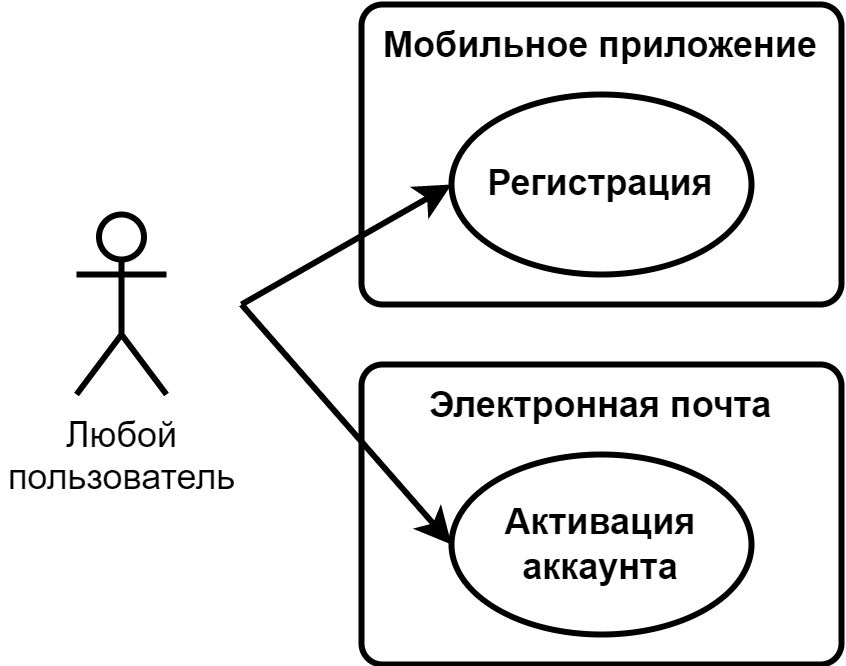
\includegraphics[width=8cm]
    {images/UML/UML_precedent_registration.png}

    \caption{Диаграмма прецедентов для регистрации}

    \label{fig:UML_precedent_registration}
\end{figure}

Смена email является важной функцией в системе,
которая предоставляет пользователям возможность изменить свой текущий email на новый.
Смена email может быть полезна по нескольким причинам.
Во-первых, пользователь может захотеть обновить свой email-адрес,
чтобы использовать более актуальный или предпочитаемый адрес электронной почты.
Во-вторых, смена email может быть необходима в случае, если текущий адрес электронной почты стал недоступным,
утерян или скомпрометирован.
В таких ситуациях пользователь должен иметь возможность обновить свой email,
чтобы продолжать пользоваться системой и получать важные уведомления.
Диаграмма прецедента <<Смены email>> изображена на рисунке~\ref{fig:UML_precedent_change_email}.

\begin{figure}[!htb]
    \centering

    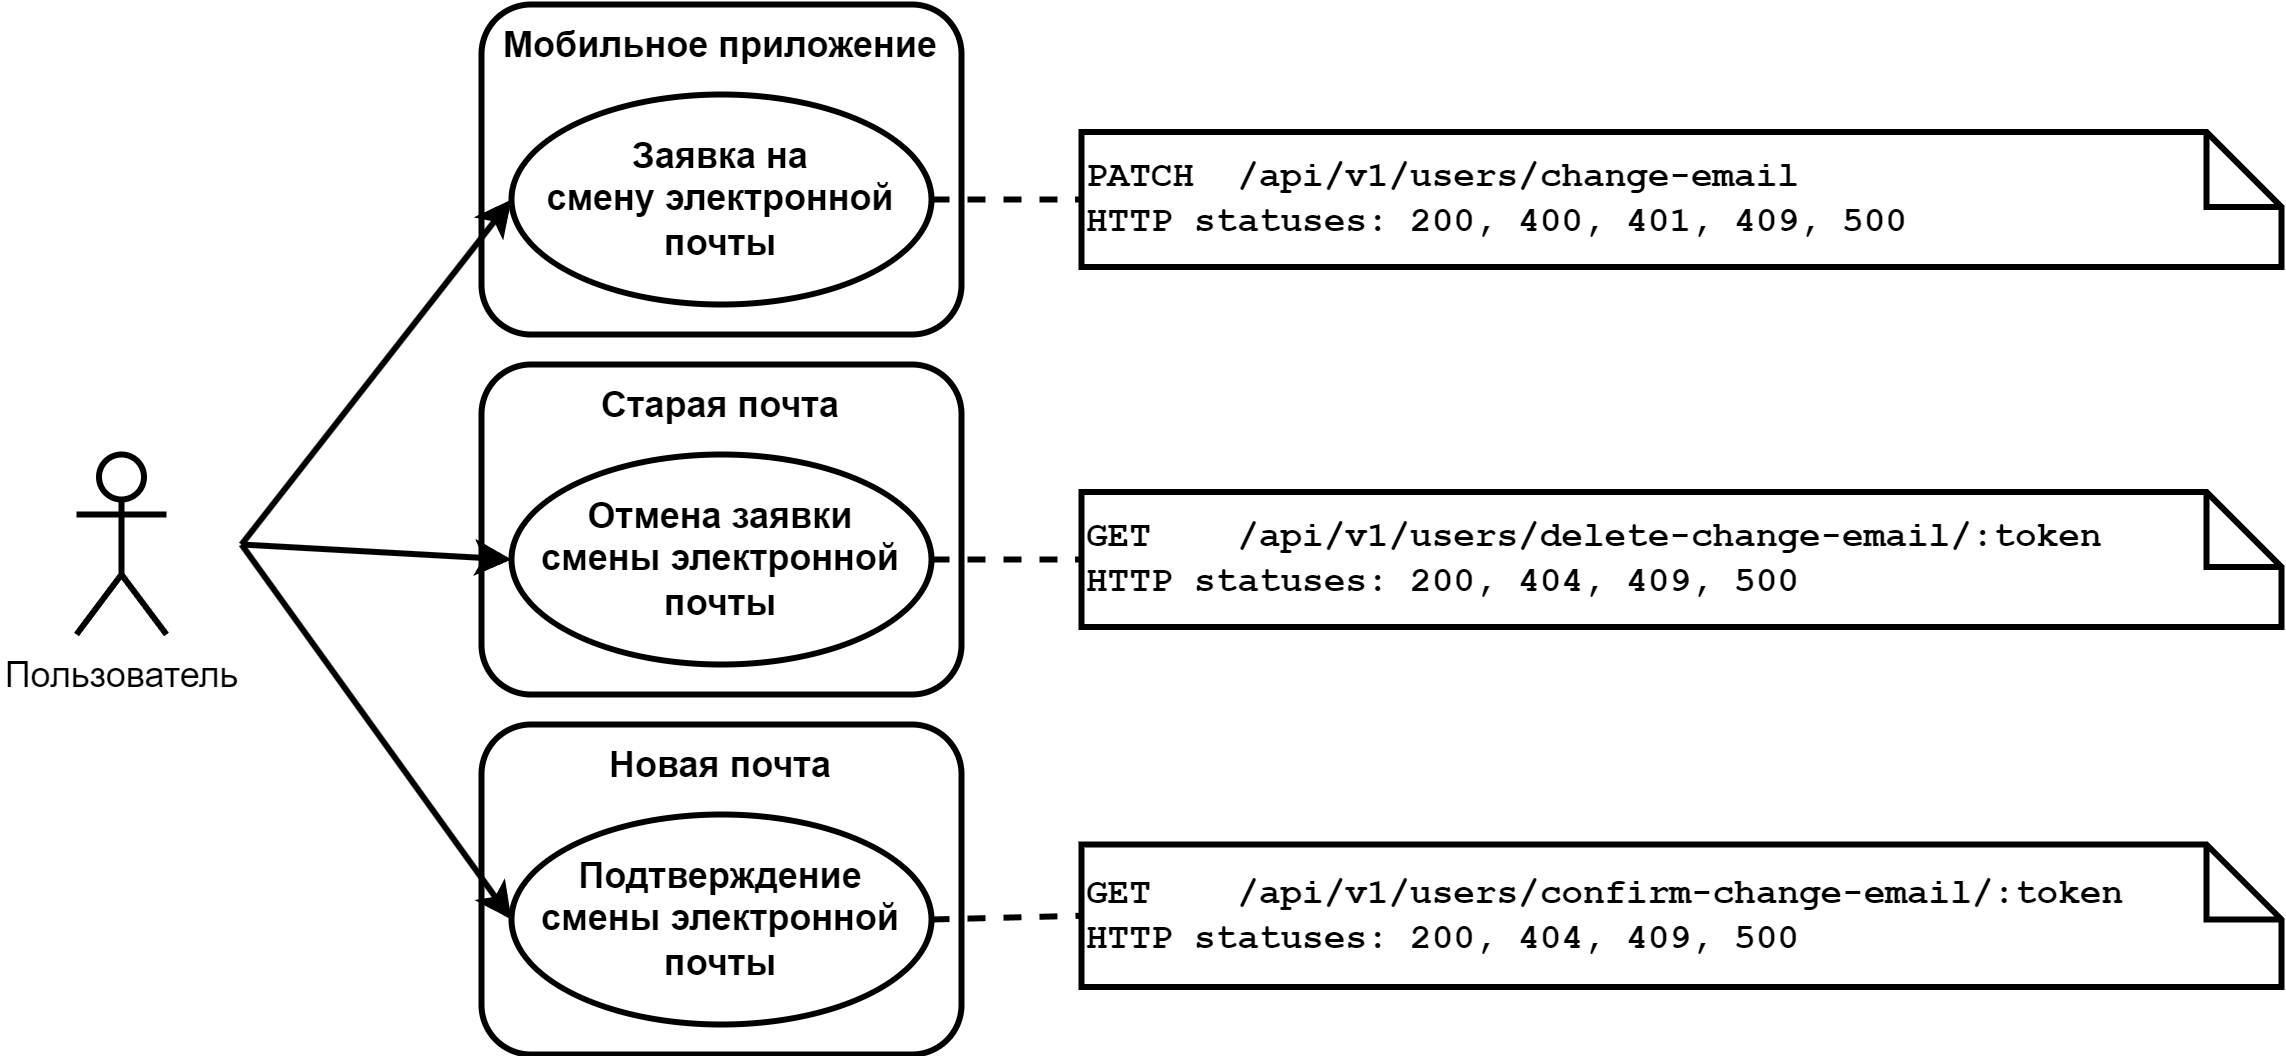
\includegraphics[width=8cm]
    {images/UML/UML_precedent_change_email.png}

    \caption{Диаграмма прецедентов для смены электронной почты}

    \label{fig:UML_precedent_change_email}
\end{figure}

Функция смены пароля играет важную роль в системе, предоставляя пользователям возможность изменить свой текущий пароль на новый.
Смена пароля является неотъемлемой частью обеспечения безопасности аккаунта пользователя.
Важно, чтобы пользователи периодически меняли свои пароли,
чтобы предотвратить несанкционированный доступ к их аккаунтам.
Эта функция позволяет пользователям обновить пароль, когда они считают,
что его безопасность может быть нарушена, или когда они хотят выбрать более надежный пароль.
Диаграмма прецедента <<Смена пароля>> изображена на рисунке~\ref{fig:UML_precedent_change_password}.

\begin{figure}[!htb]
    \centering

    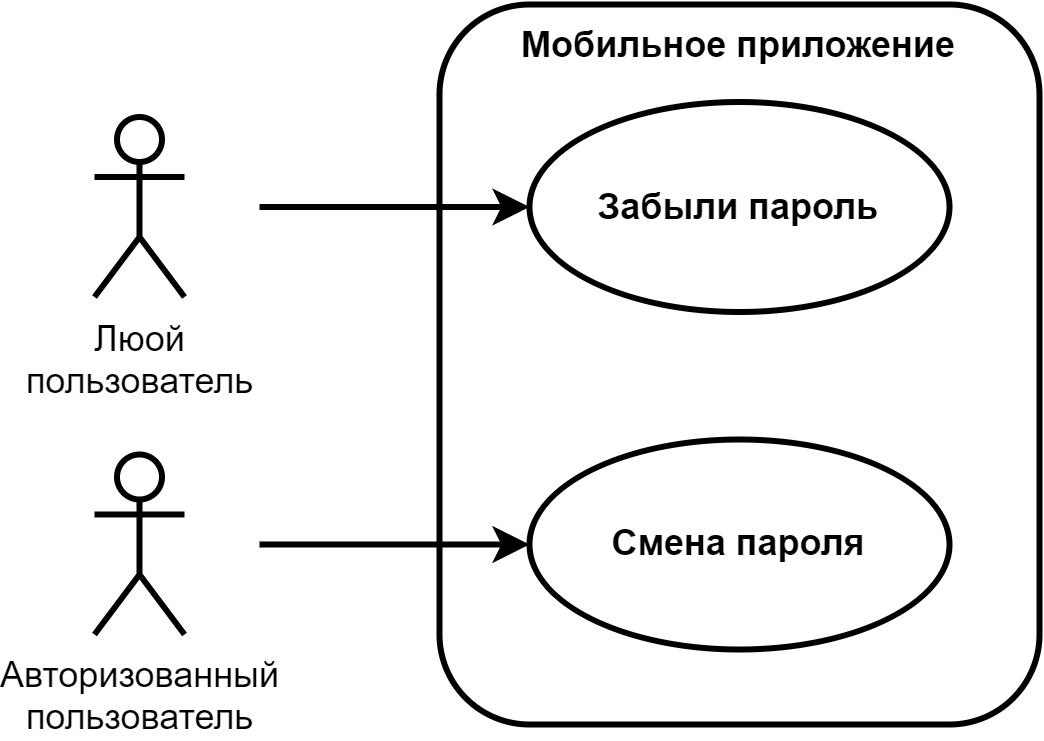
\includegraphics[height=5.5cm]
    {images/UML/UML_precedent_change_password.png}

    \caption{Диаграмма прецедентов для смены пароля}

    \label{fig:UML_precedent_change_password}
\end{figure}

Вход в аккаунт позволяет пользователям получить доступ к персонализированному контенту, функциям и привилегиям,
доступным только для авторизованных пользователей.
Это может включать в себя возможность добавления товаров в избранное, оформления заказов,
просмотра персональной информации и так далее.
Диаграмма прецедента <<Вход в аккаунт>> изображена на рисунке~\ref{fig:UML_precedent_sessions}.

\begin{figure}[!htb]
    \centering

    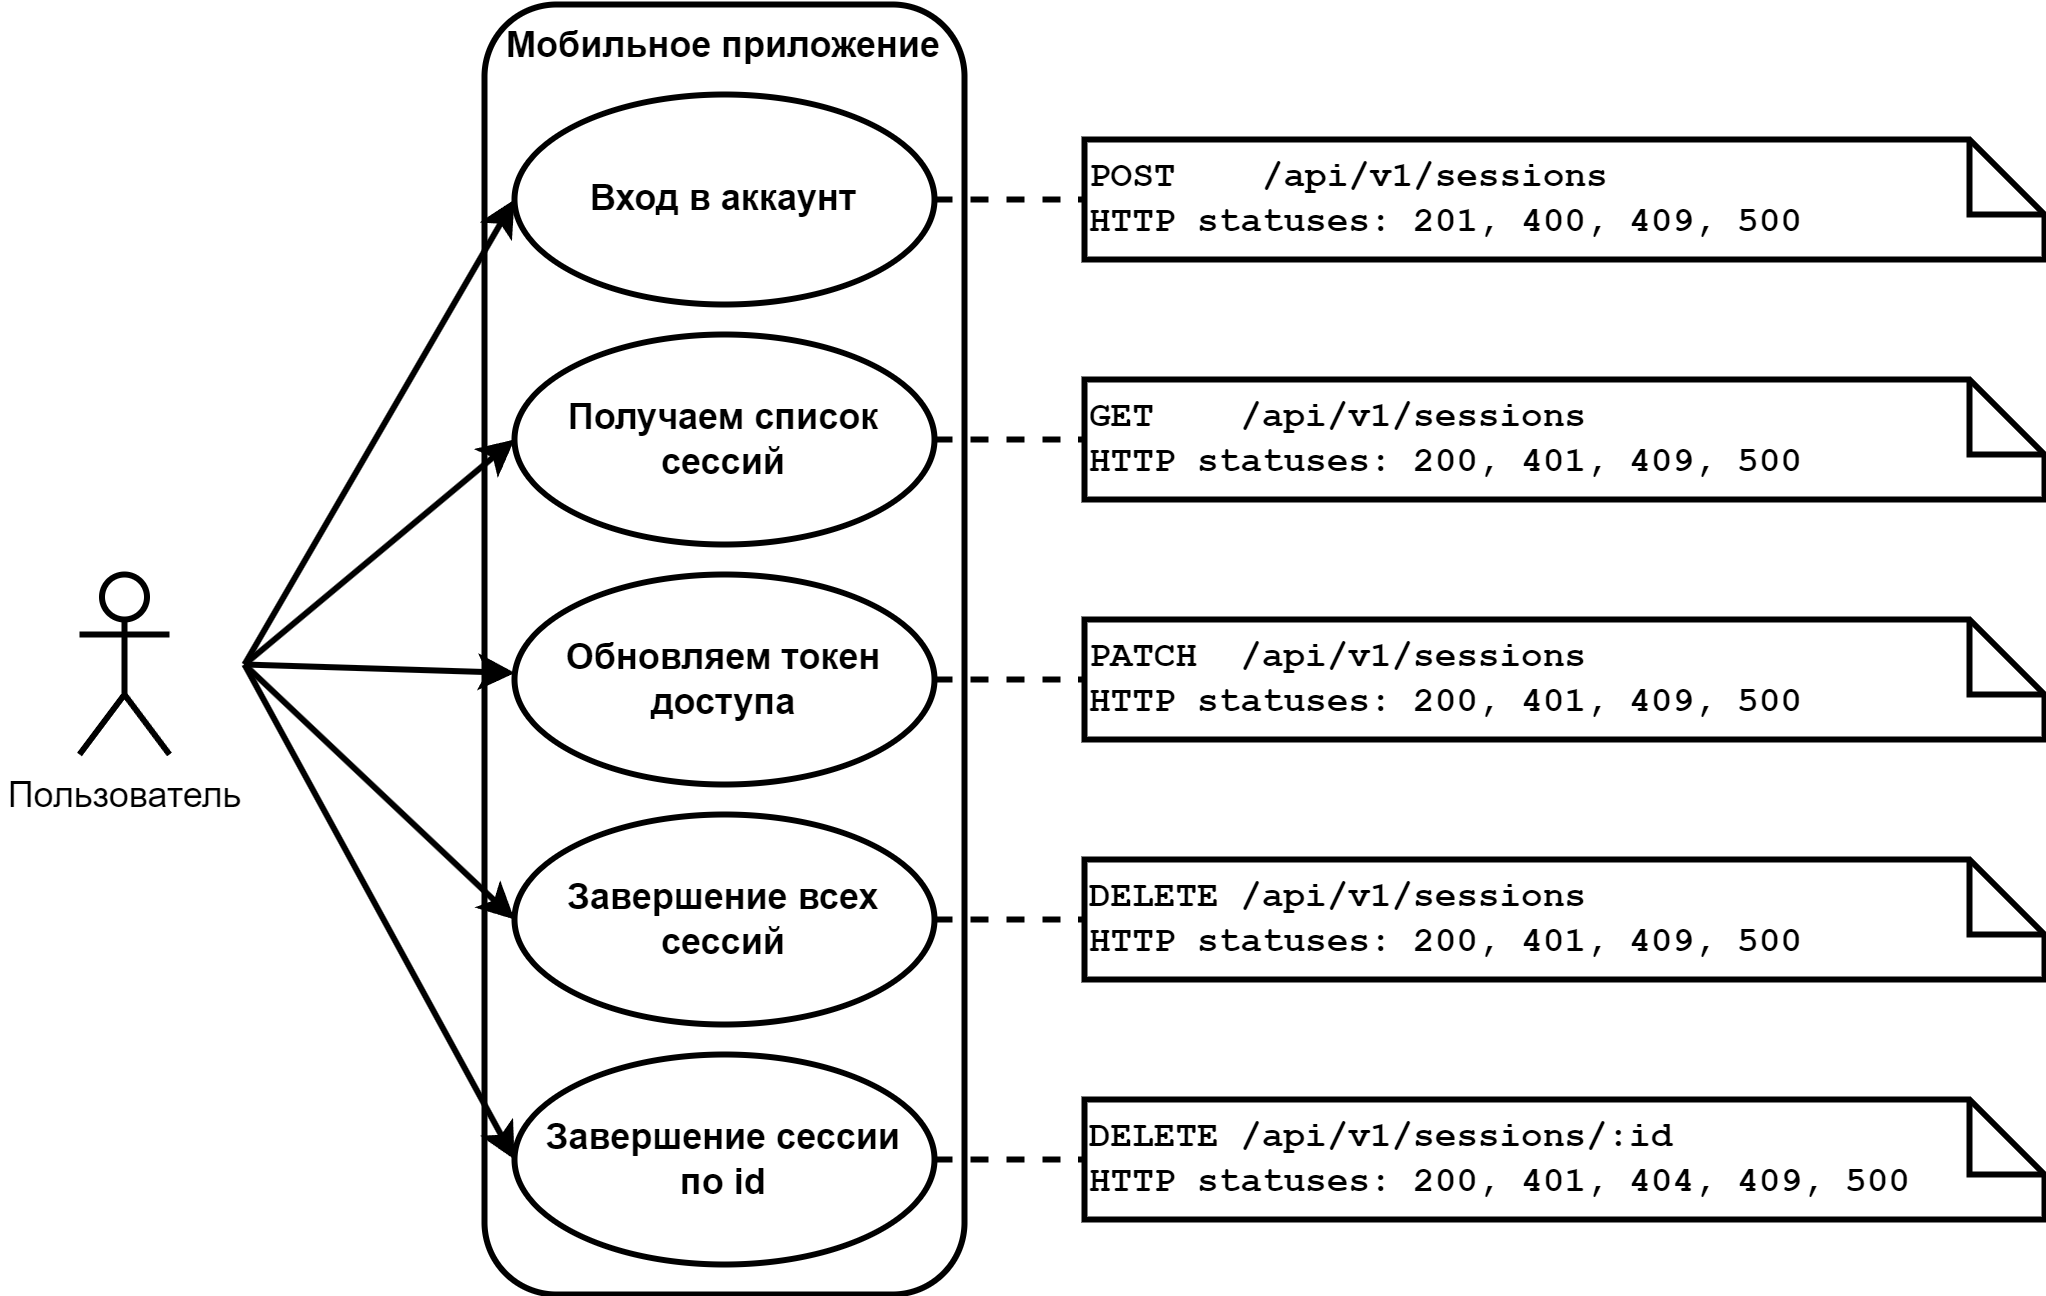
\includegraphics[height=9.2cm]
    {images/UML/UML_precedent_sessions.png}

    \caption{Диаграмма прецедентов для входа в аккаунт}

    \label{fig:UML_precedent_sessions}
\end{figure}

Разбиение товаров по брендам при оформлении заказа имеет несколько причин и преимуществ.
Во-первых, такой подход облегчает навигацию по каталогу и позволяет покупателям легко найти и выбрать товары
от определенных производителей.
Во-вторых, разделение товаров по брендам упрощает фильтрацию и сортировку товаров,
что позволяет покупателям быстро находить нужные им товары.
Это также способствует удобству использования интернет-магазина и повышает уровень удовлетворенности клиентов.
Таким образом, разбиение товаров по брендам при заказе является полезной функцией,
которая упрощает процесс выбора и покупки товаров.
Диаграмма прецедента <<Манипуляции с брендом>> изображена на рисунке~\ref{fig:UML_precedent_item_brands}.

\begin{figure}[!htb]
    \centering

    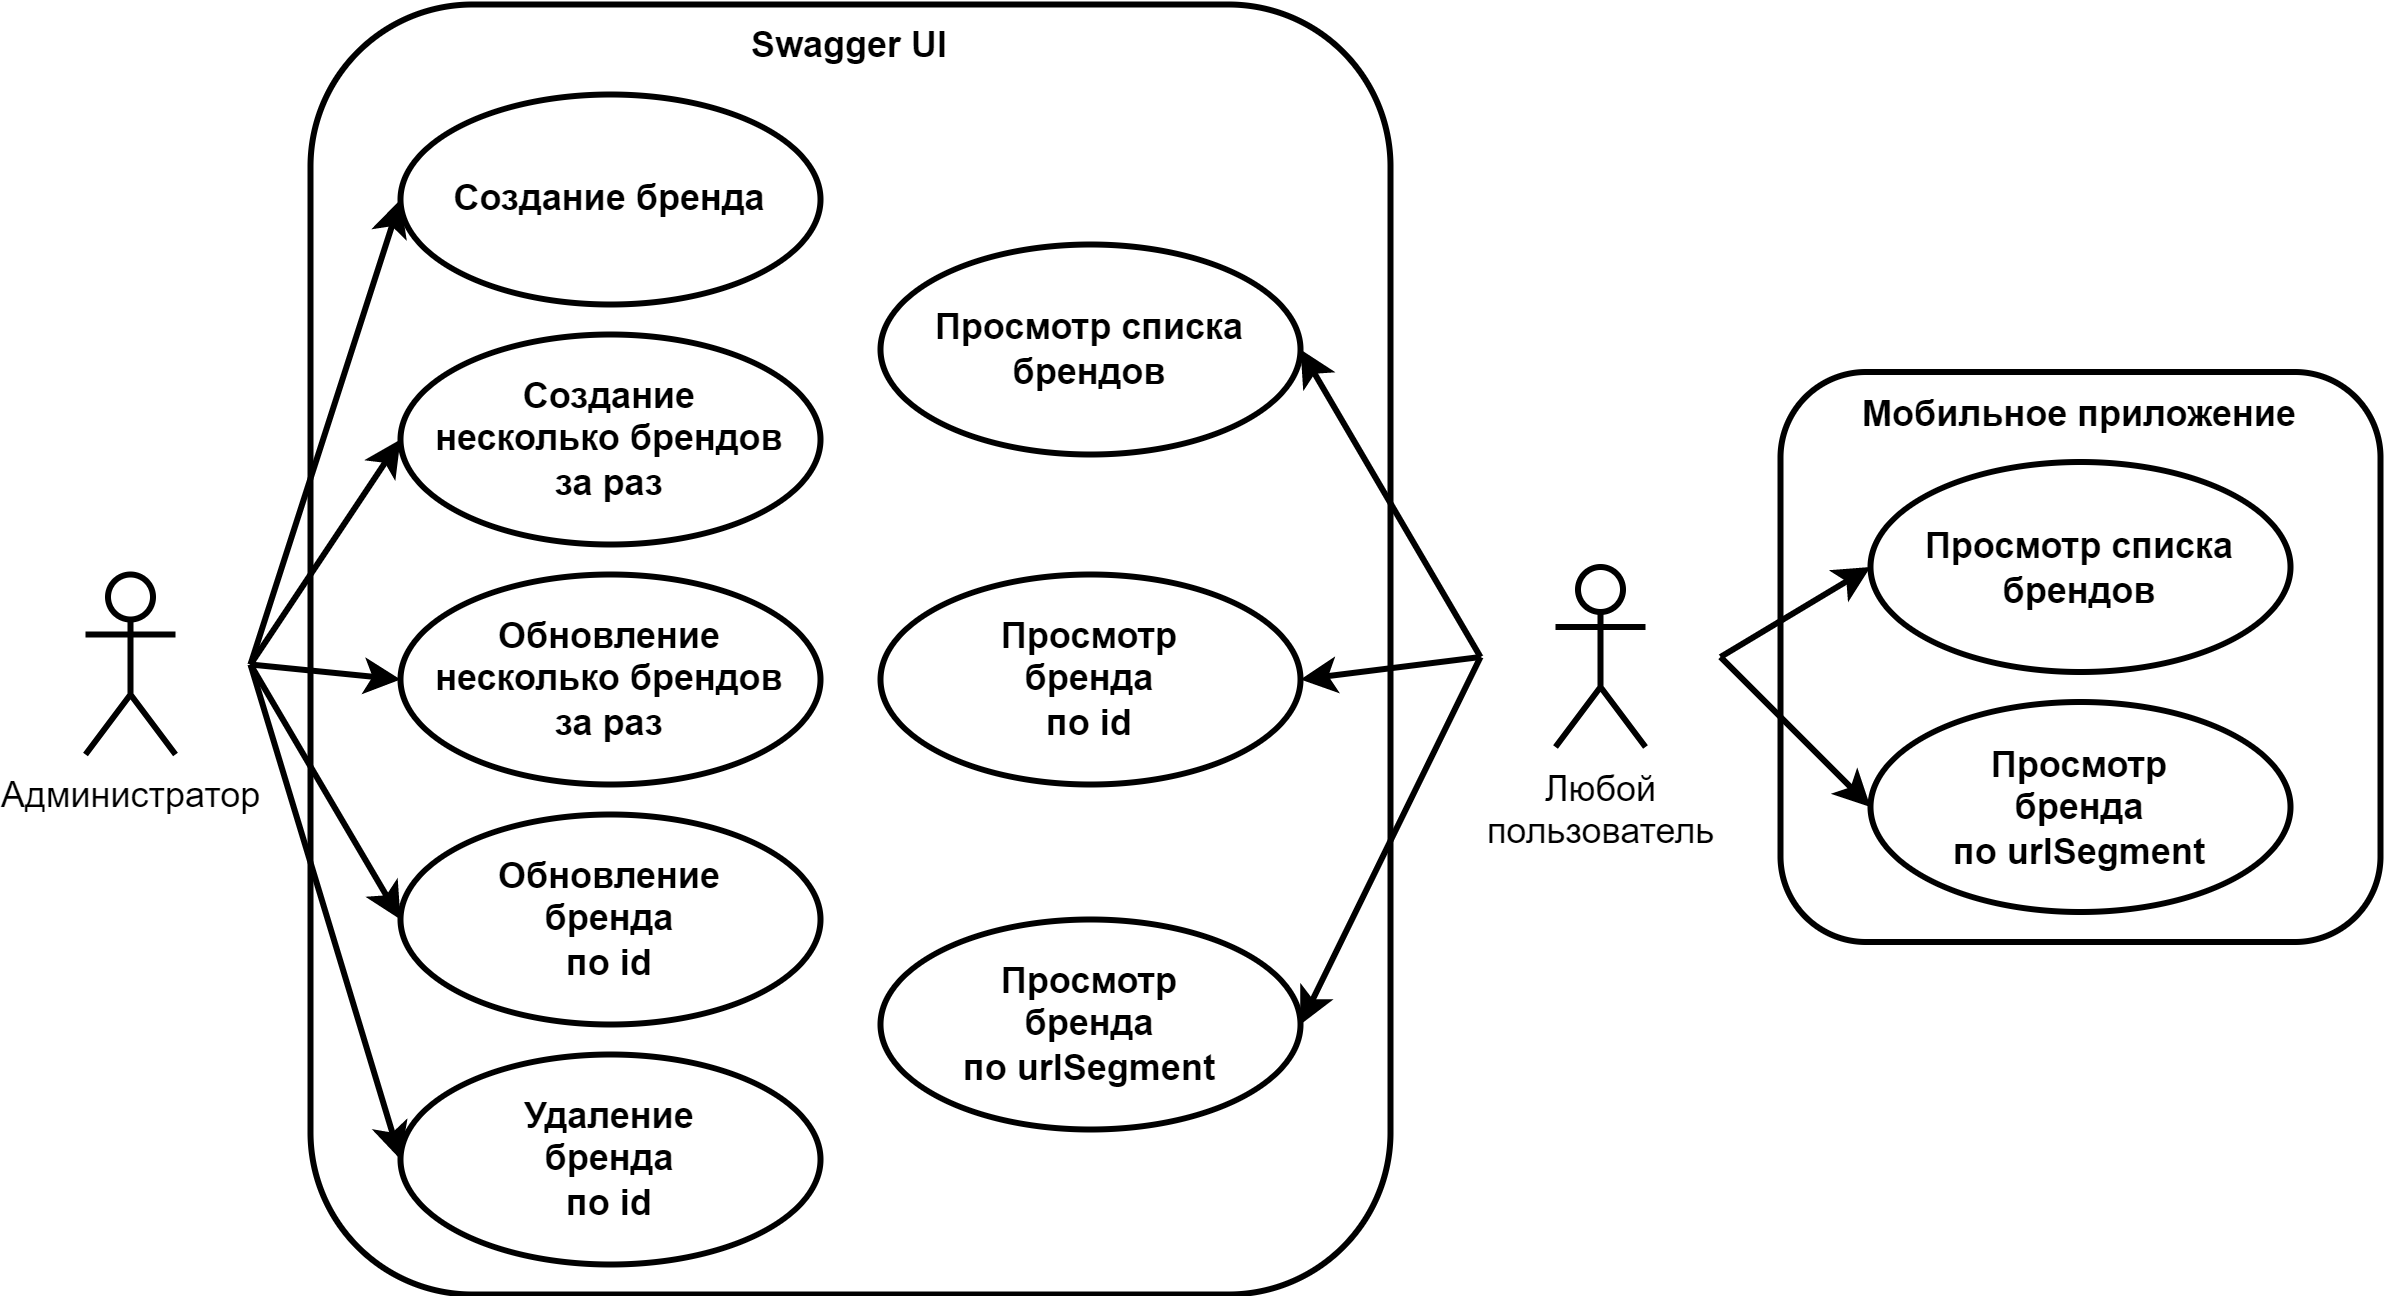
\includegraphics[height=9.2cm]
    {images/UML/UML_precedent_item_brands.png}

    \caption{Диаграмма прецедентов для манипуляции с брендами}

    \label{fig:UML_precedent_item_brands}
\end{figure}
Категории товаров представляют собой логическую группировку товаров в интернет-магазинах.
Они используются для классификации товарного ассортимента по общим характеристикам.
Категории помогают пользователям легко найти нужные товары, а также упрощают навигацию по магазину.
Диаграмма прецедента <<Манипуляции с категориями>> изображена на рисунке~\ref{fig:UML_precedent_item_categories}.

\begin{figure}[!htb]
    \centering

    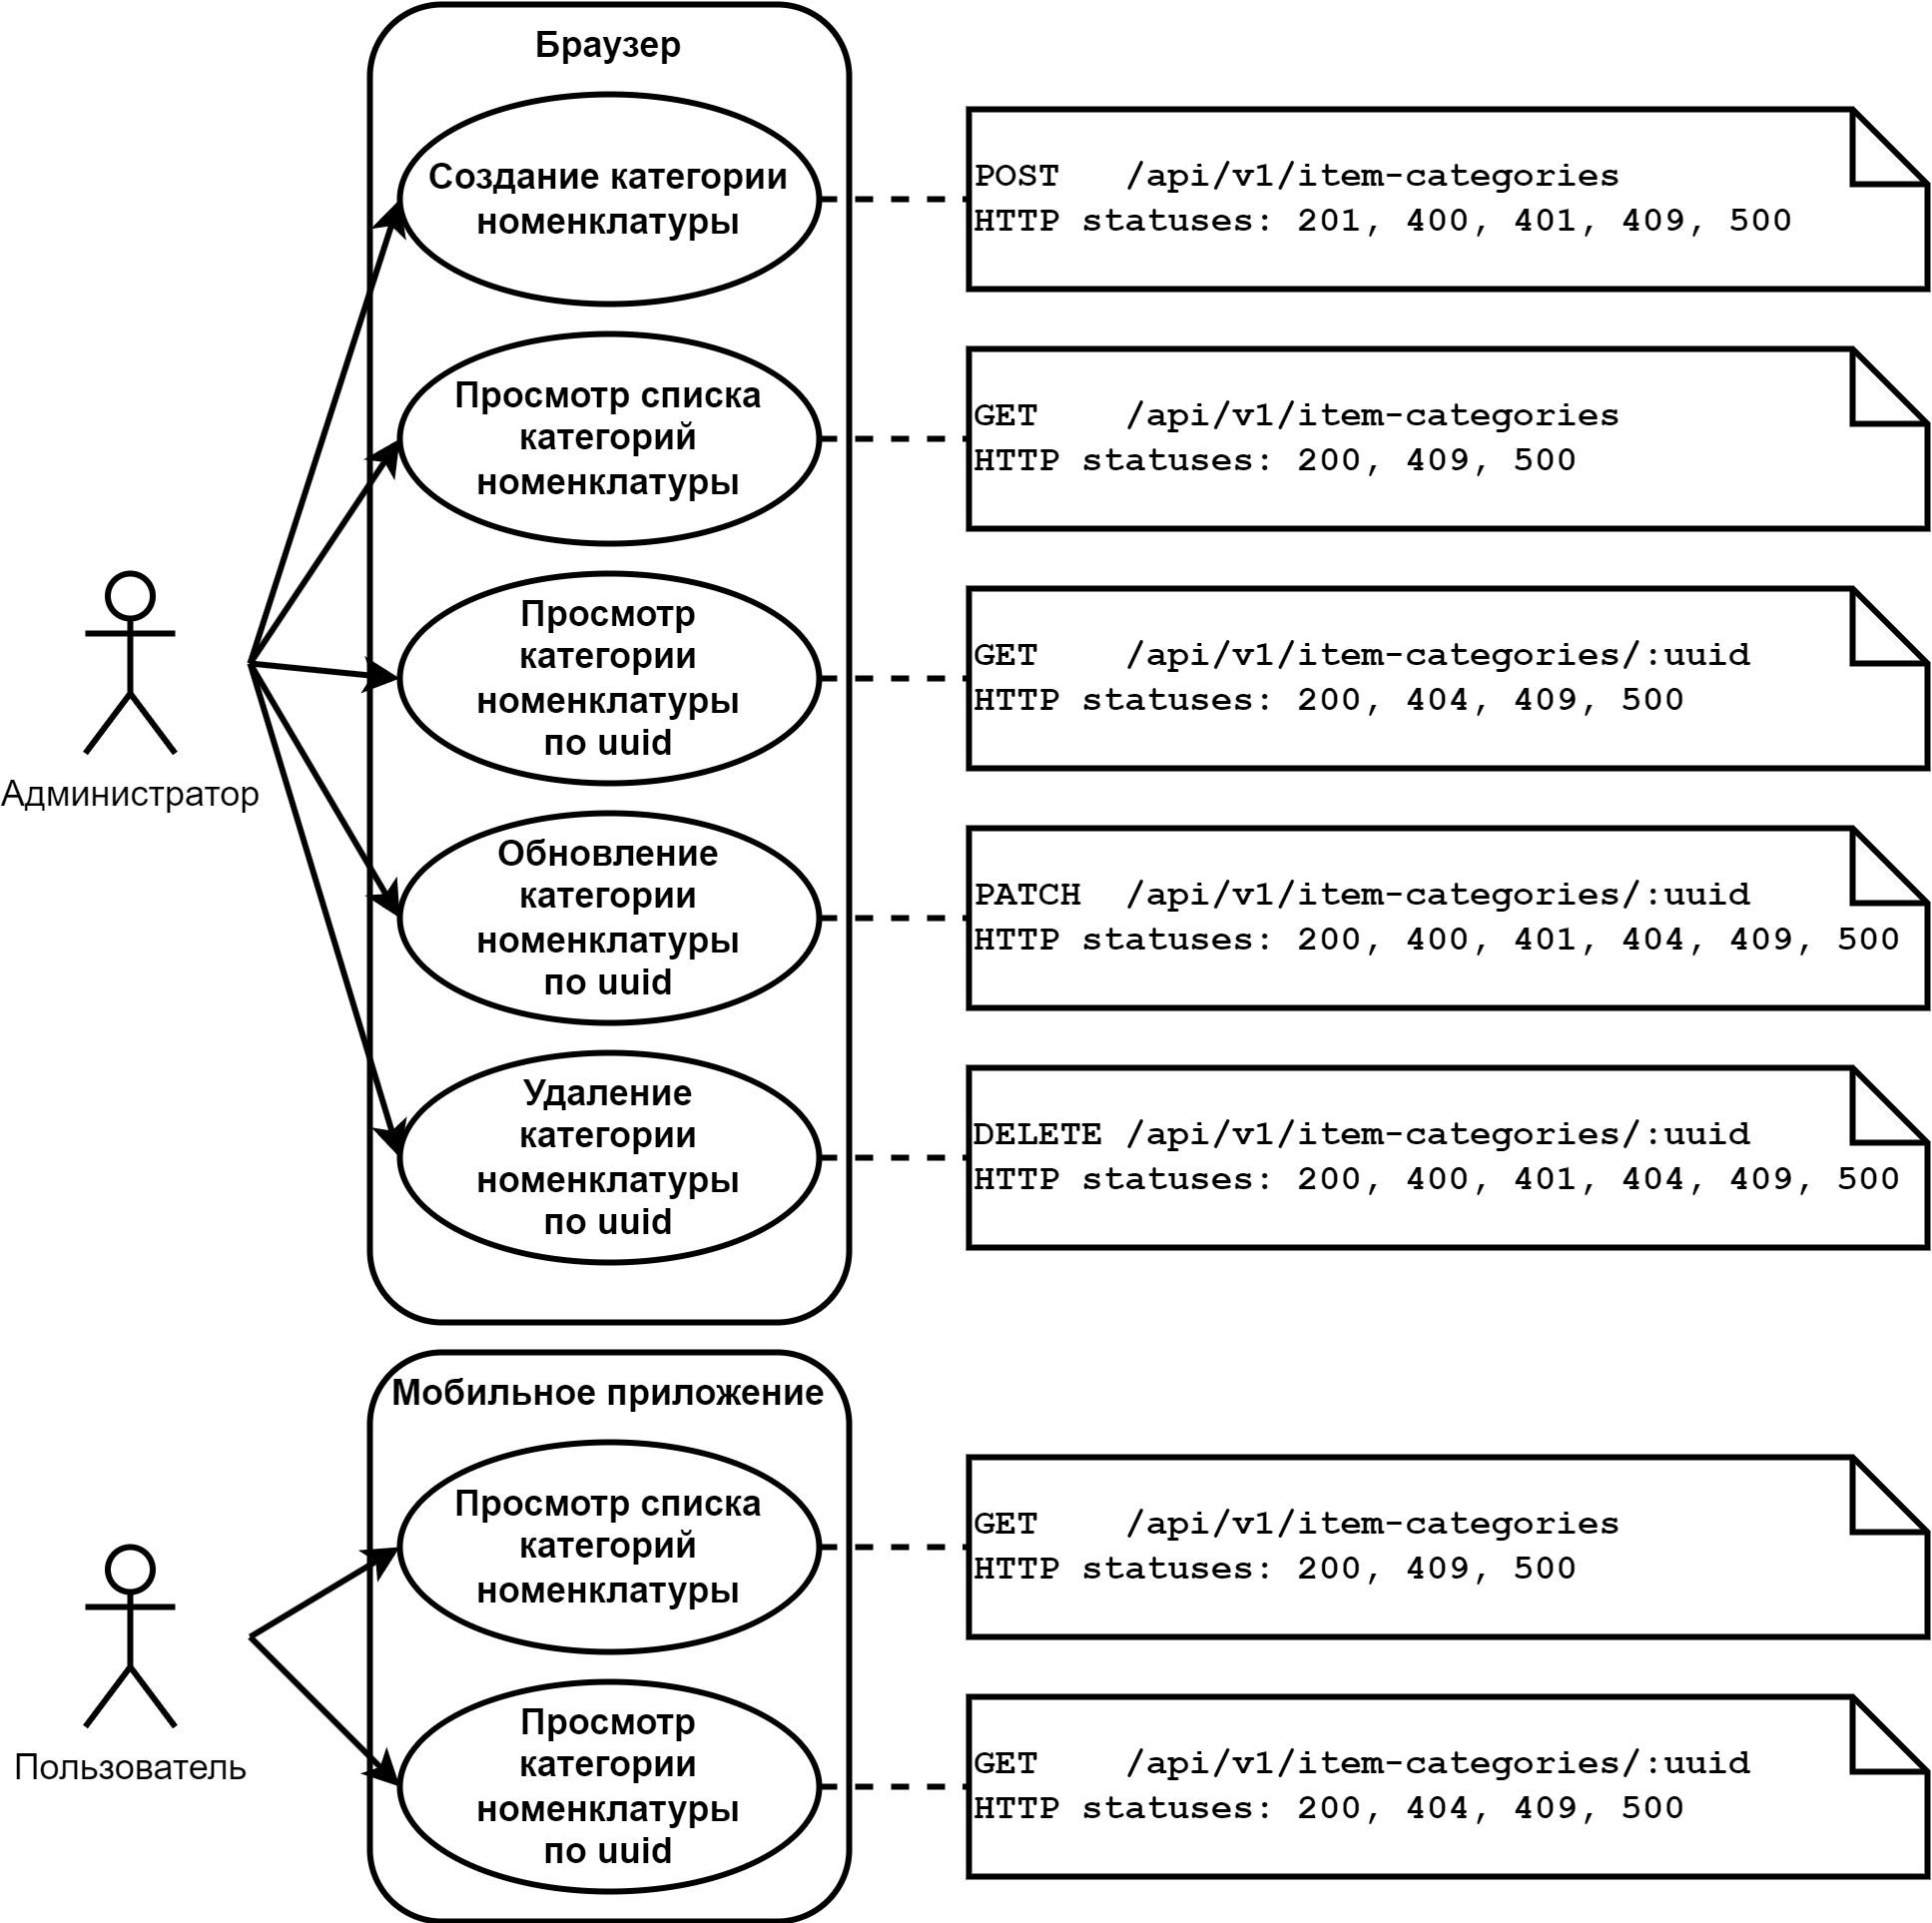
\includegraphics[height=9.2cm]
    {images/UML/UML_precedent_item_categories.png}

    \caption{Диаграмма прецедентов для манипуляции с категориями}

    \label{fig:UML_precedent_item_categories}
\end{figure}

Номенклатура - это термин, который обычно используется для обозначения полного списка товаров или продукции,
доступных в определенной организации.
Номенклатура обычно включает в себя информацию о каждом товаре, включая его название, код, описание, характеристики, цену
которые могут быть полезными для идентификации и классификации товаров.
Диаграмма прецедента <<Манипуляции с номенклатурой>> изображена на рисунке~\ref{fig:UML_precedent_items}.

\begin{figure}[!htb]
    \centering

    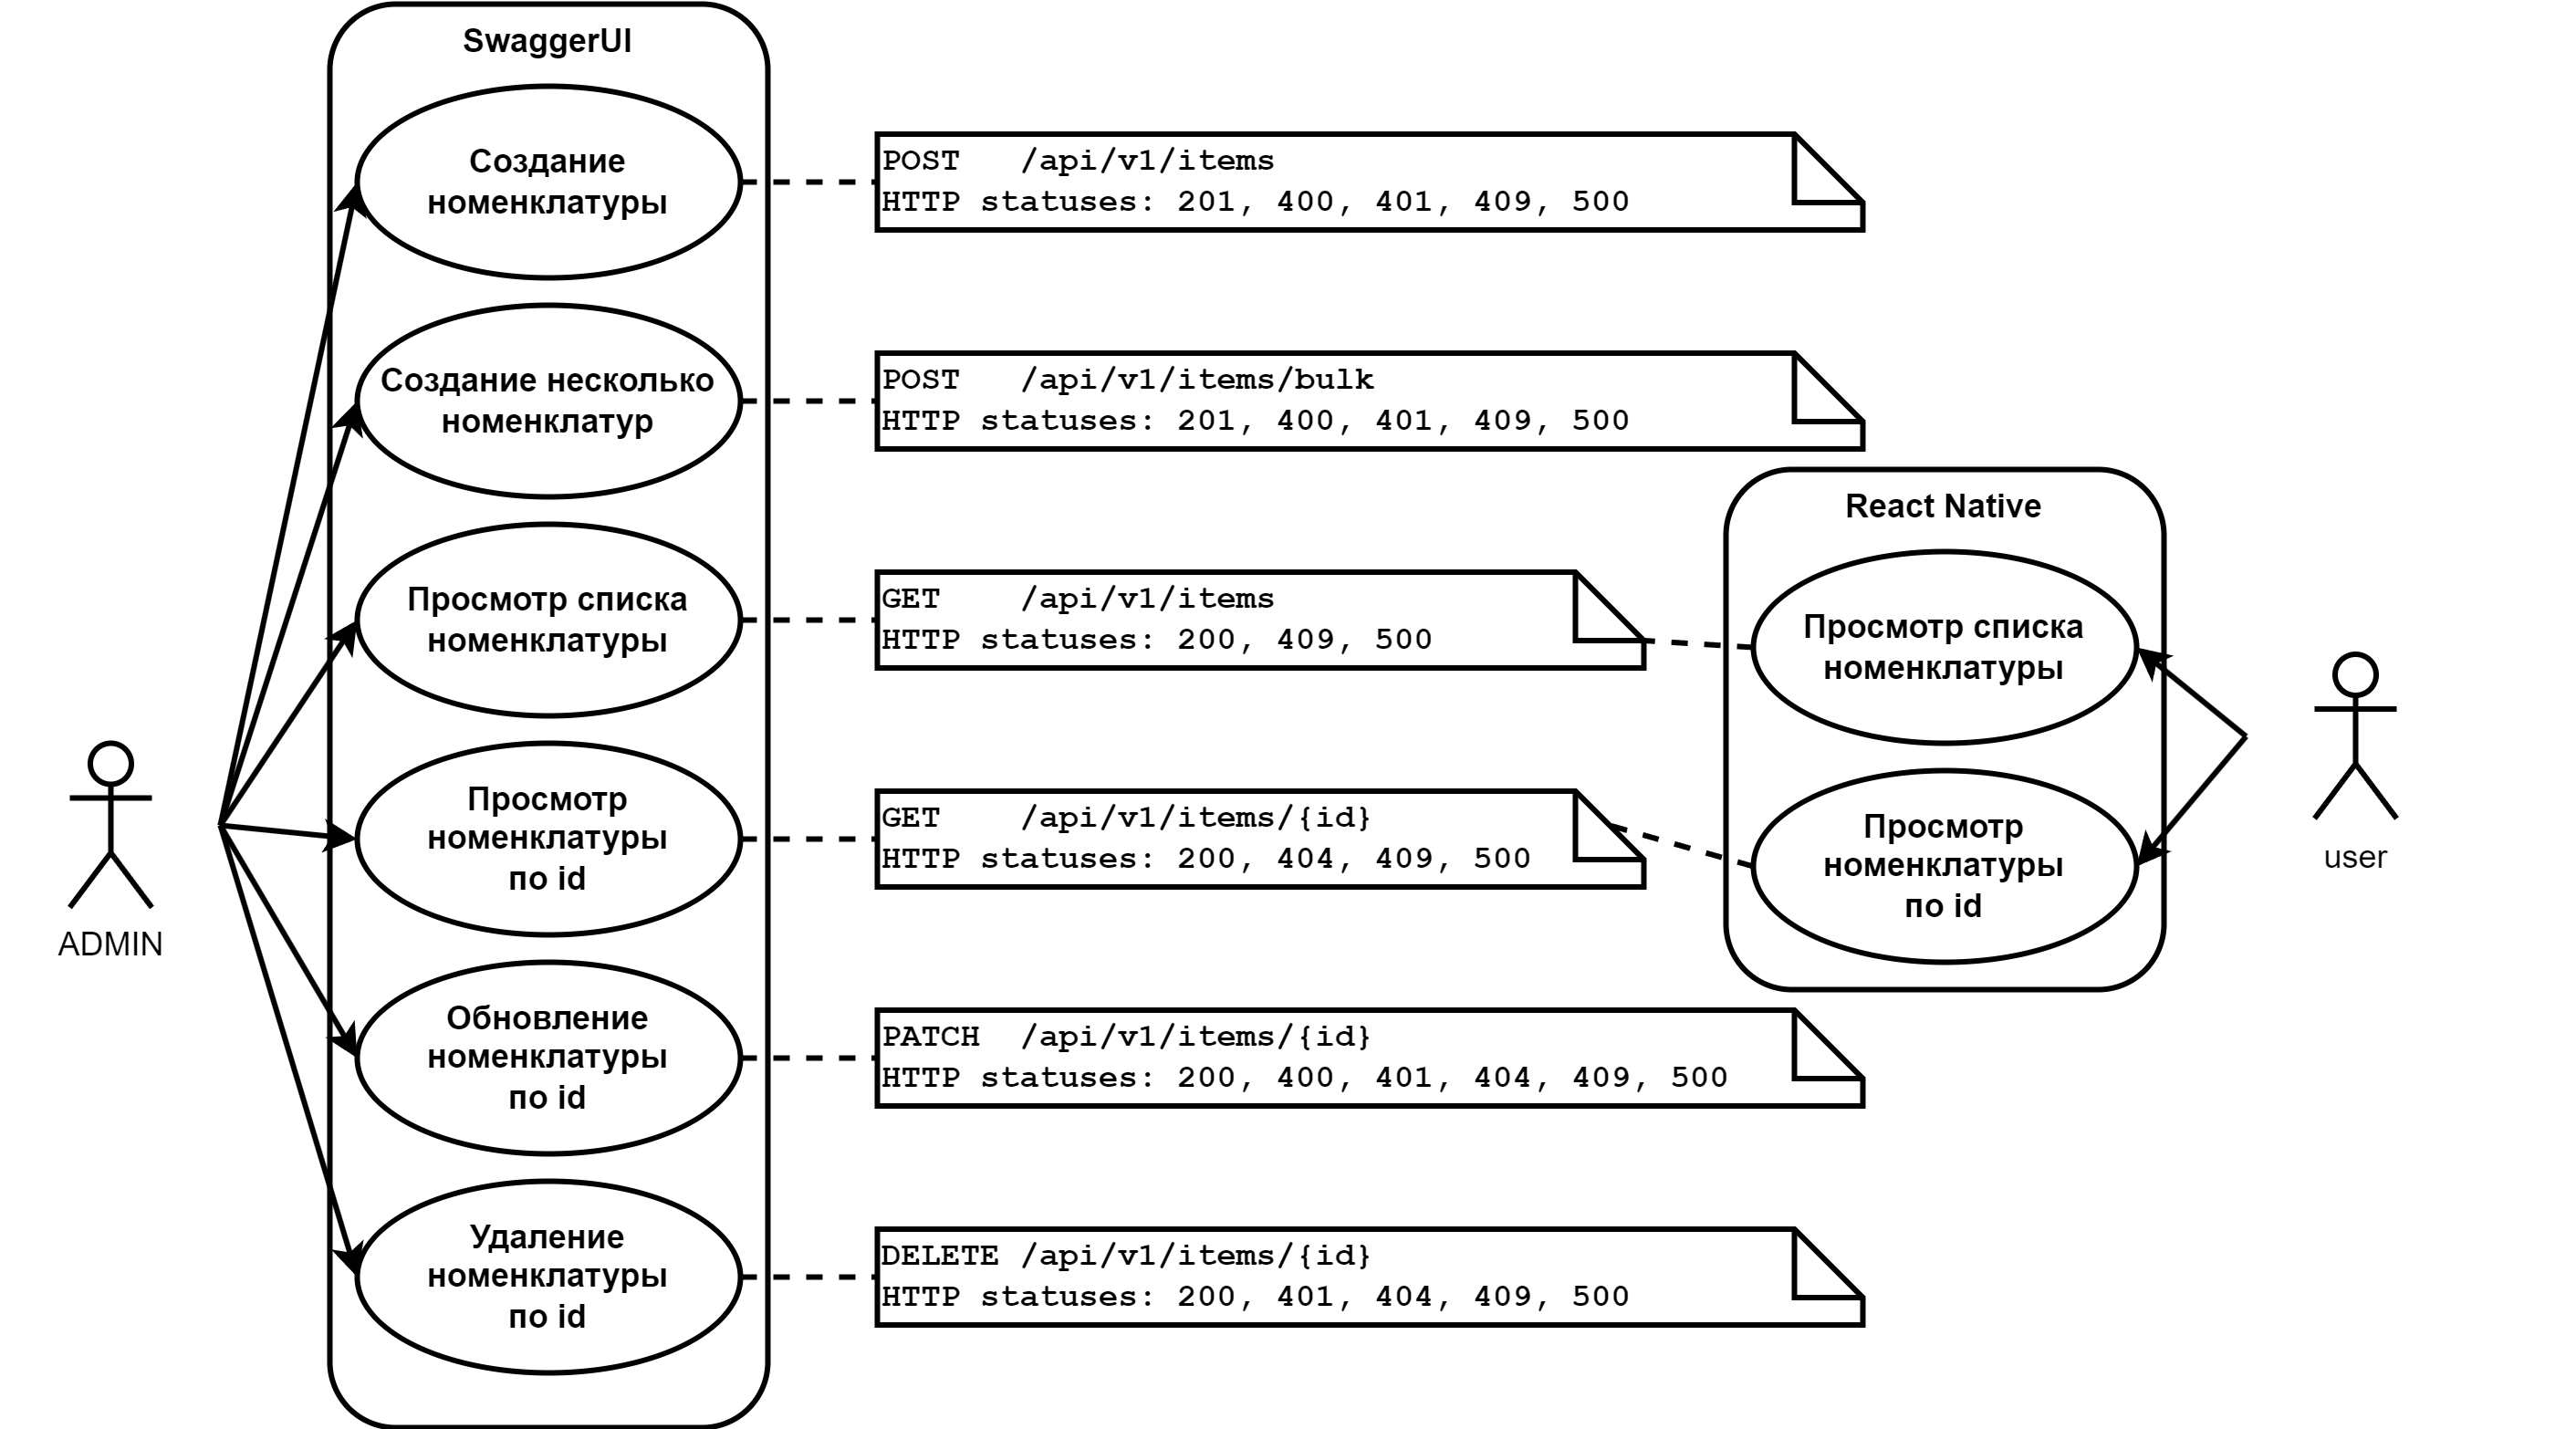
\includegraphics[height=11cm]
    {images/UML/UML_precedent_items.png}

    \caption{Диаграмма прецедентов для манипуляции с номеклатурой}

    \label{fig:UML_precedent_items}
\end{figure}

Характеристика номенклатуры - это дополнительная информация о товаре,
которая описывает его особенности, свойства, параметры или другие специфические атрибуты.
Она предоставляет дополнительную детализацию о товаре, которая может быть полезна для покупателей и других заинтересованных сторон.
Характеристики номенклатуры могут включать такие данные, как размеры, цвет, материал, вес, производительность, технические параметры, срок гарантии и другие сведения,
которые помогают более точно определить товар и сравнить его с другими.
Наличие отдельного справочника для характеристик номенклатуры позволяет легко добавлять новые характеристики
или изменять существующие без необходимости вносить изменения в основную структуру номенклатуры.
Это способствует гибкости и масштабируемости системы учета и управления товарами.
Диаграмма прецедента <<Манипуляции с характеристиками>> изображена на рисунке~\ref{fig:UML_precedent_item_characteristics}.

\begin{figure}[!htb]
    \centering

    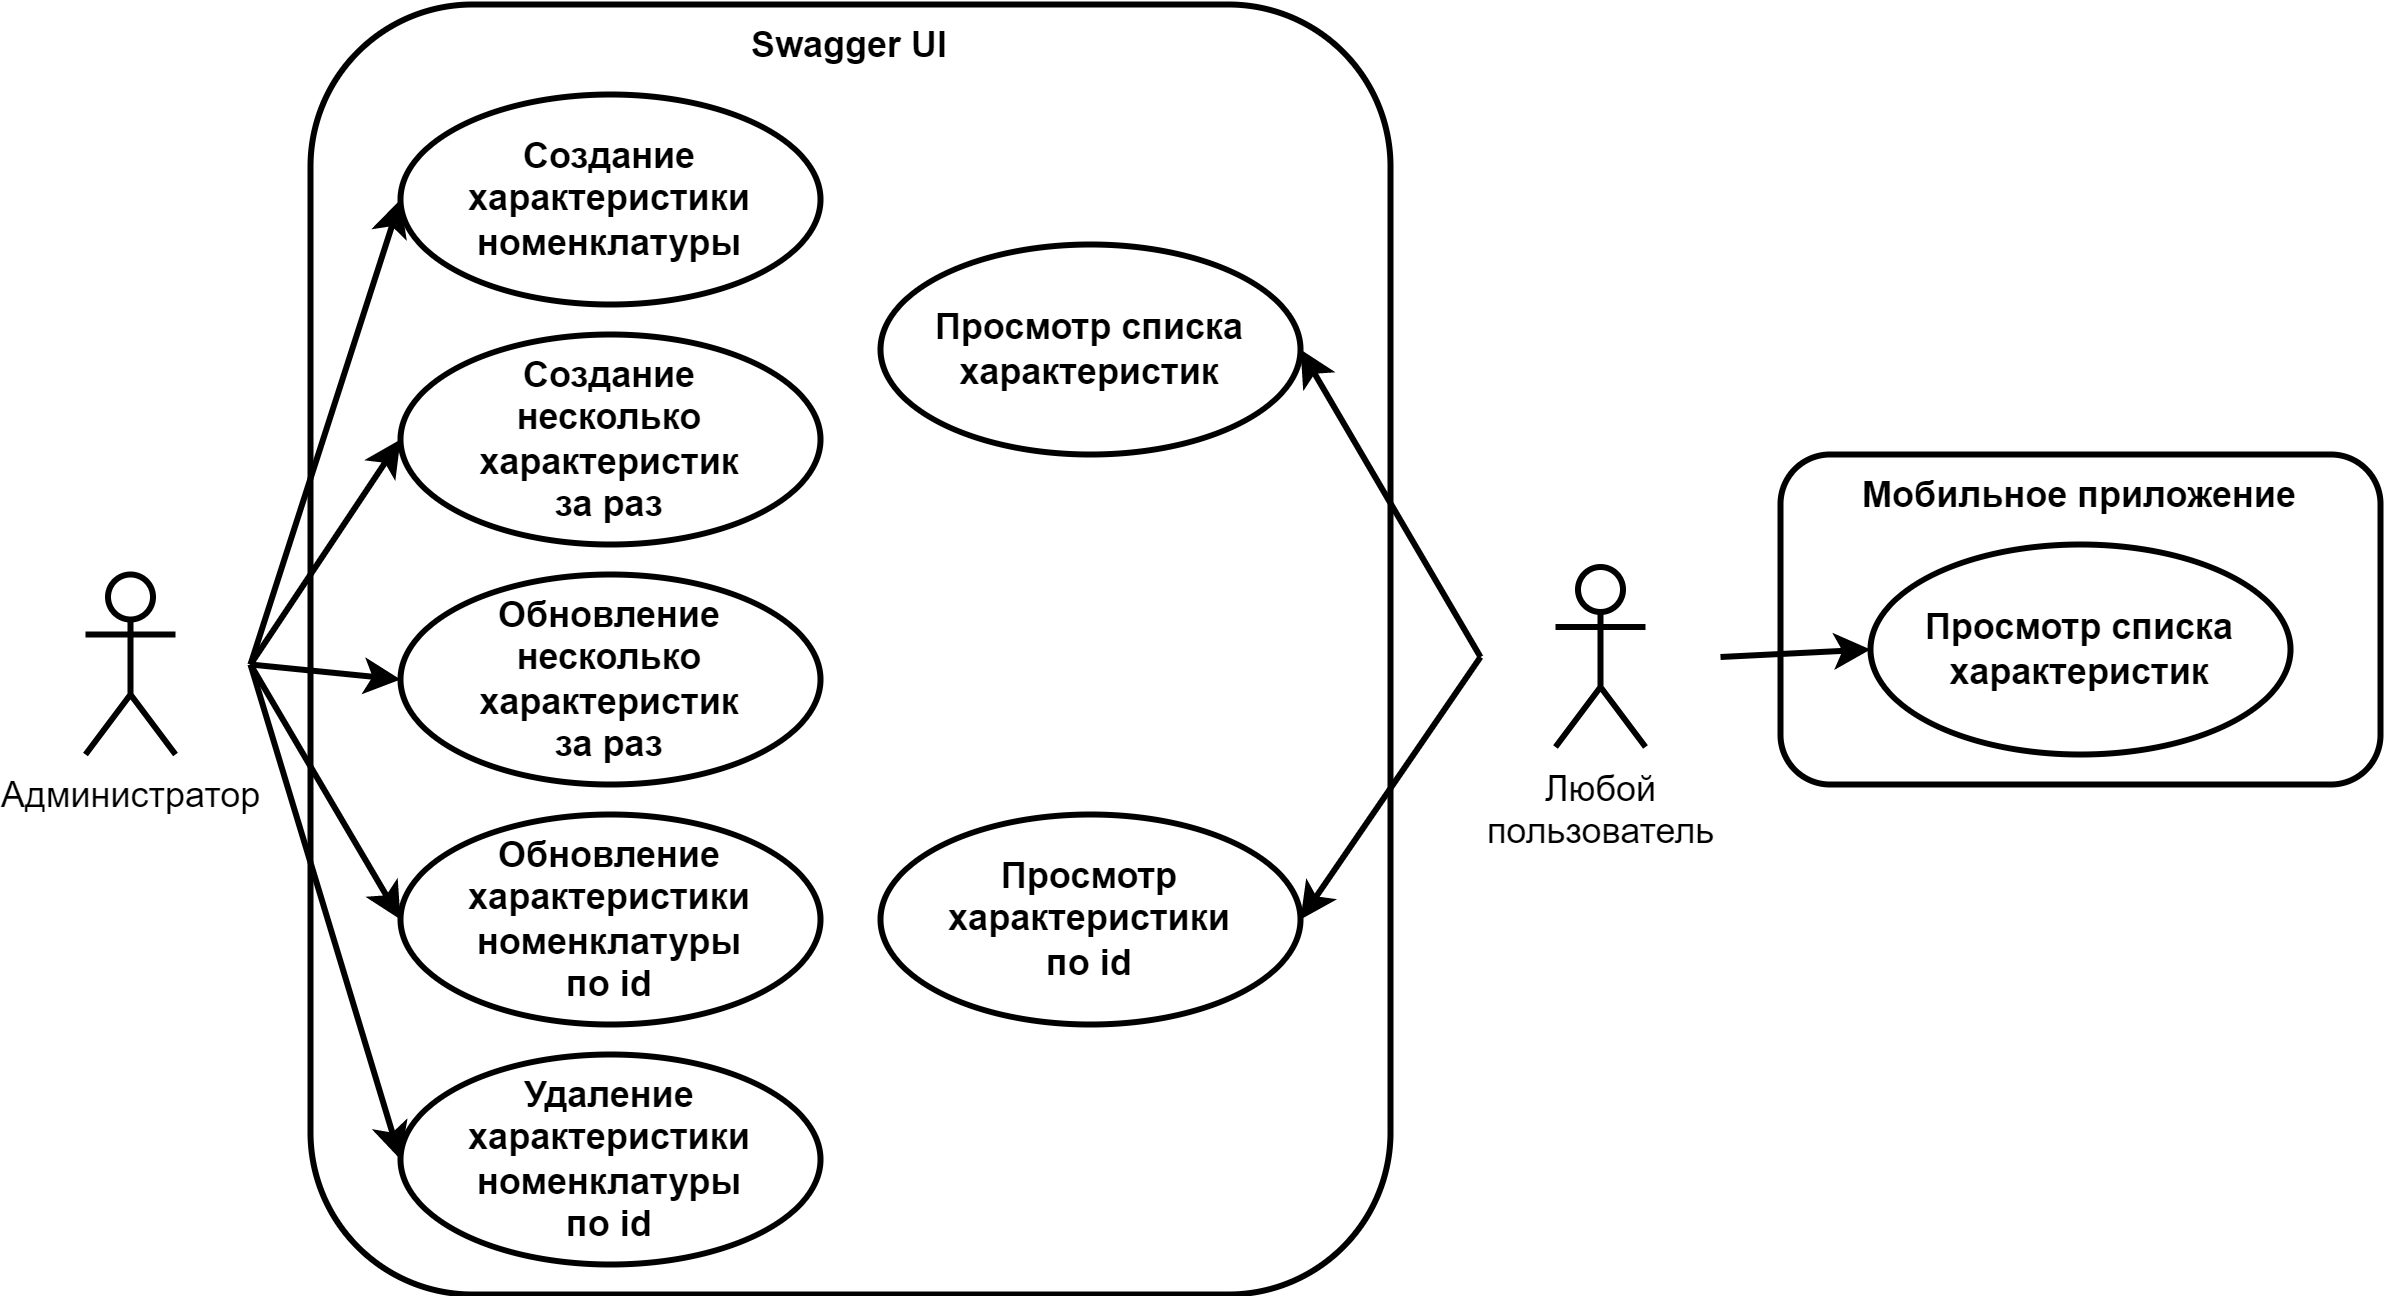
\includegraphics[height=9cm]
    {images/UML/UML_precedent_item_characteristics.png}

    \caption{Диаграмма прецедентов для манипуляции с характеристиками}

    \label{fig:UML_precedent_item_characteristics}
\end{figure}

Оформление заявки - это процесс, при котором клиент оформляет официальный запрос на приобретение товаров.
Оно осуществляется на основе товаров, которые находятся в корзине или выбраны клиентом для покупки.
Диаграмма прецедента <<Оформление заявки>> изображена на рисунке~\ref{fig:UML_precedent_order_items}.

\begin{figure}[!htb]
    \centering

    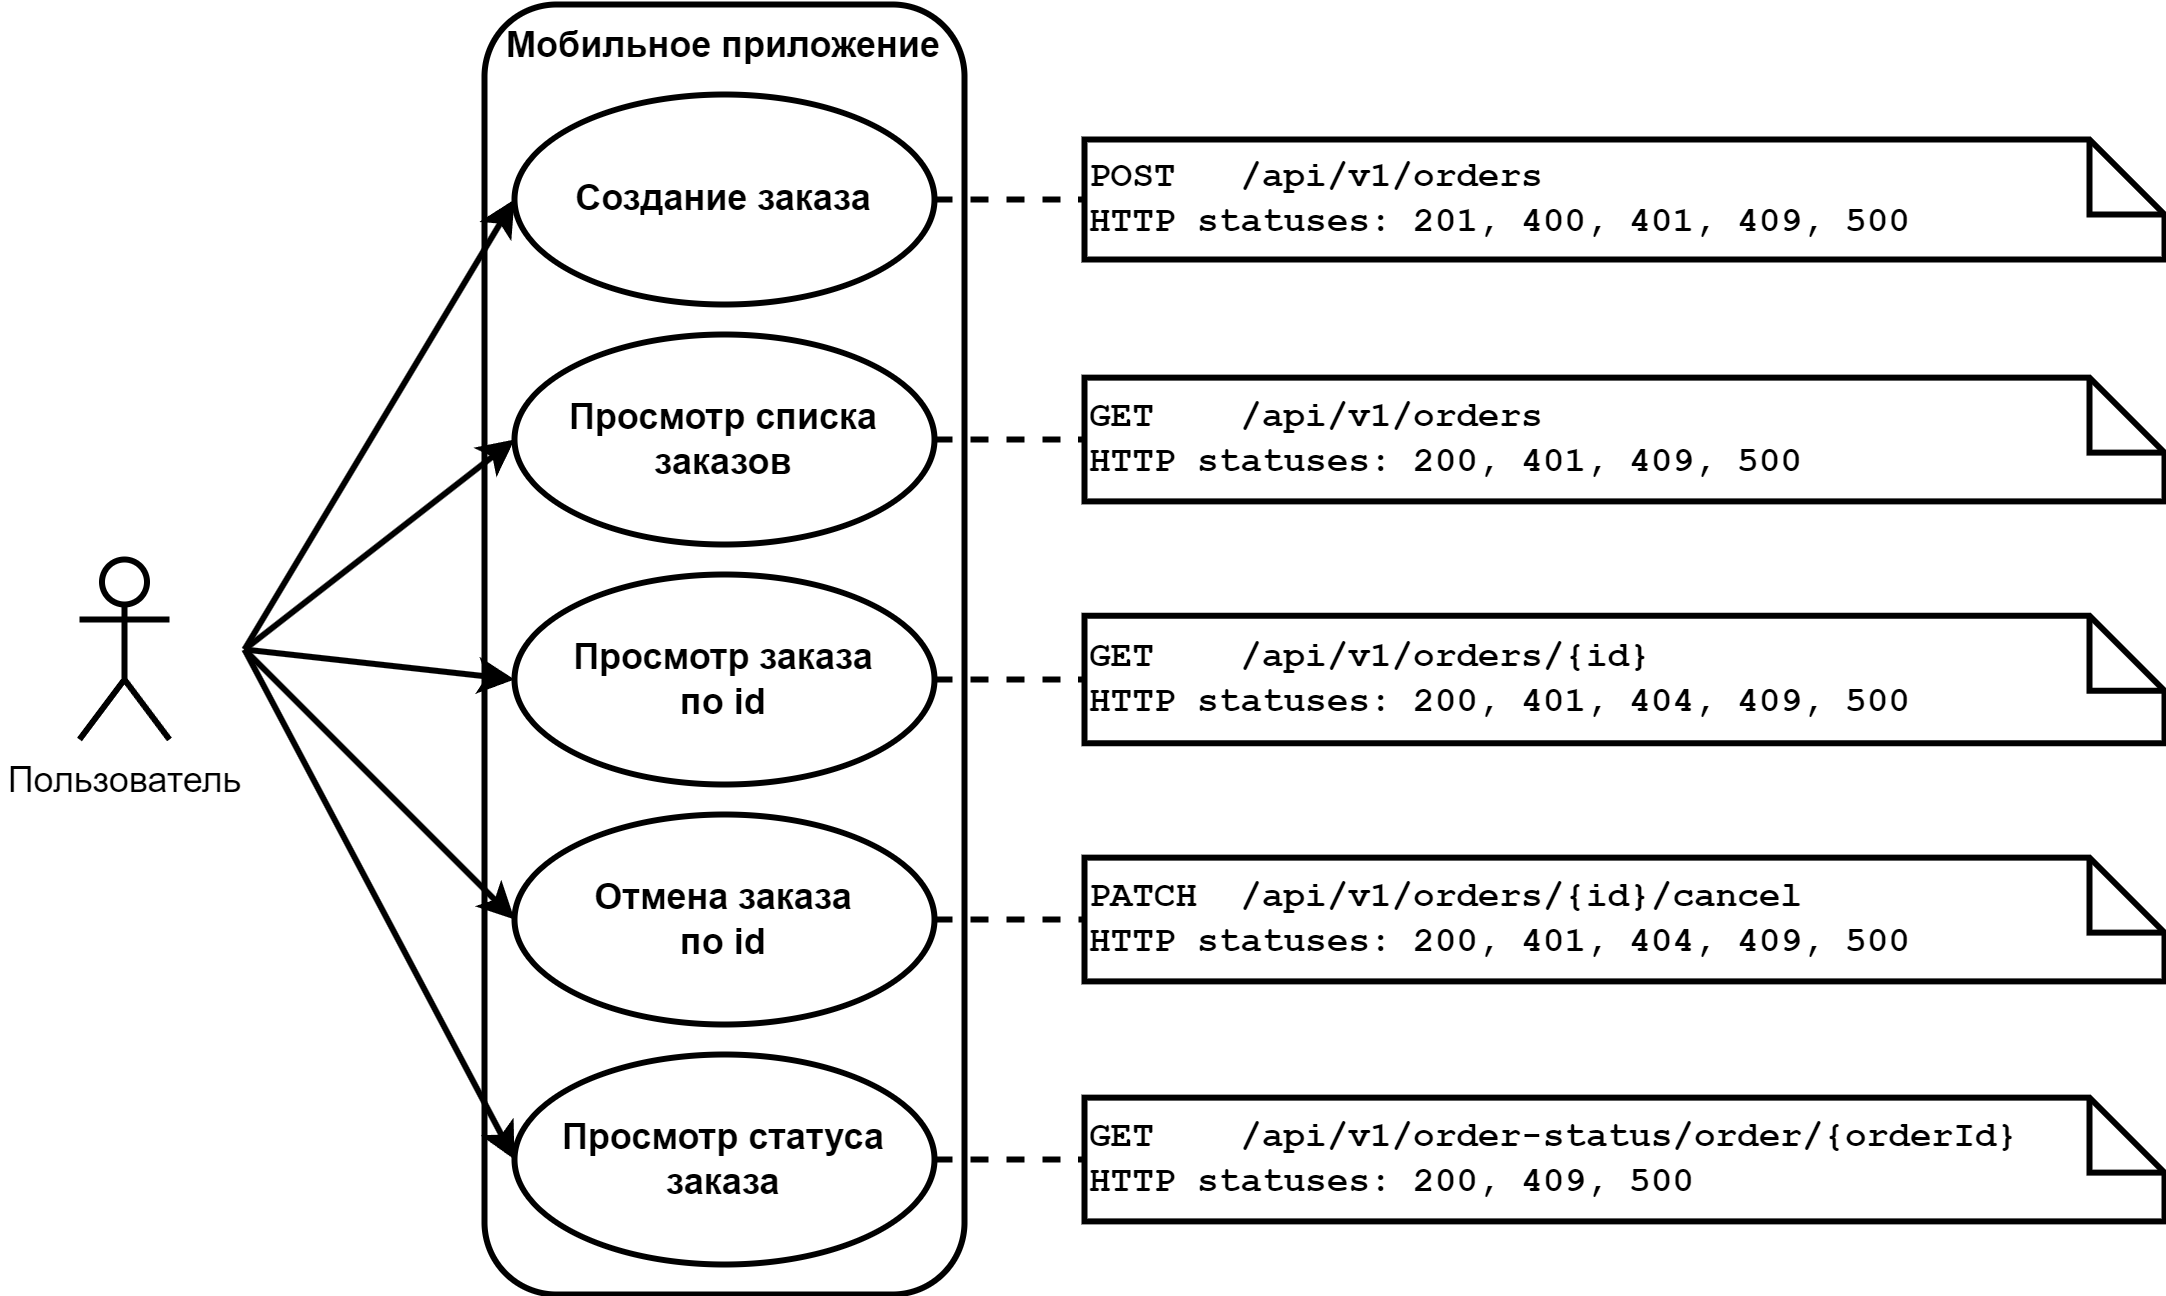
\includegraphics[height=9cm]
    {images/UML/UML_precedent_order_items.png}

    \caption{Диаграмма прецедентов для заявки отбора товаров}

    \label{fig:UML_precedent_order_items}
\end{figure}

Каталоги, прайс-листы и сертификаты - это данные, которые можно представить в виде статей.
В каждой статье можено прикрепить ссылки на соответствующие файлы,
чтобы пользователь мог легко получить доступ к документам.
Страница контактов - это статья, где вы можно предоставить пользователю различные способы связи с организацией.
Здесь можно указать электронные почты, телефоны и даже популярные мессенджеры, такие как WhatsApp, Skype, Telegram и Viber.
Пользователи смогут найти все необходимые контактные данные и связаться прямо из приложения, сэкономив время и усилия.
Диаграмма прецедента <<Манипуляции со статьями>> изображена на рисунке~\ref{fig:UML_precedent_articles}.

\begin{figure}[!htb]
    \centering

    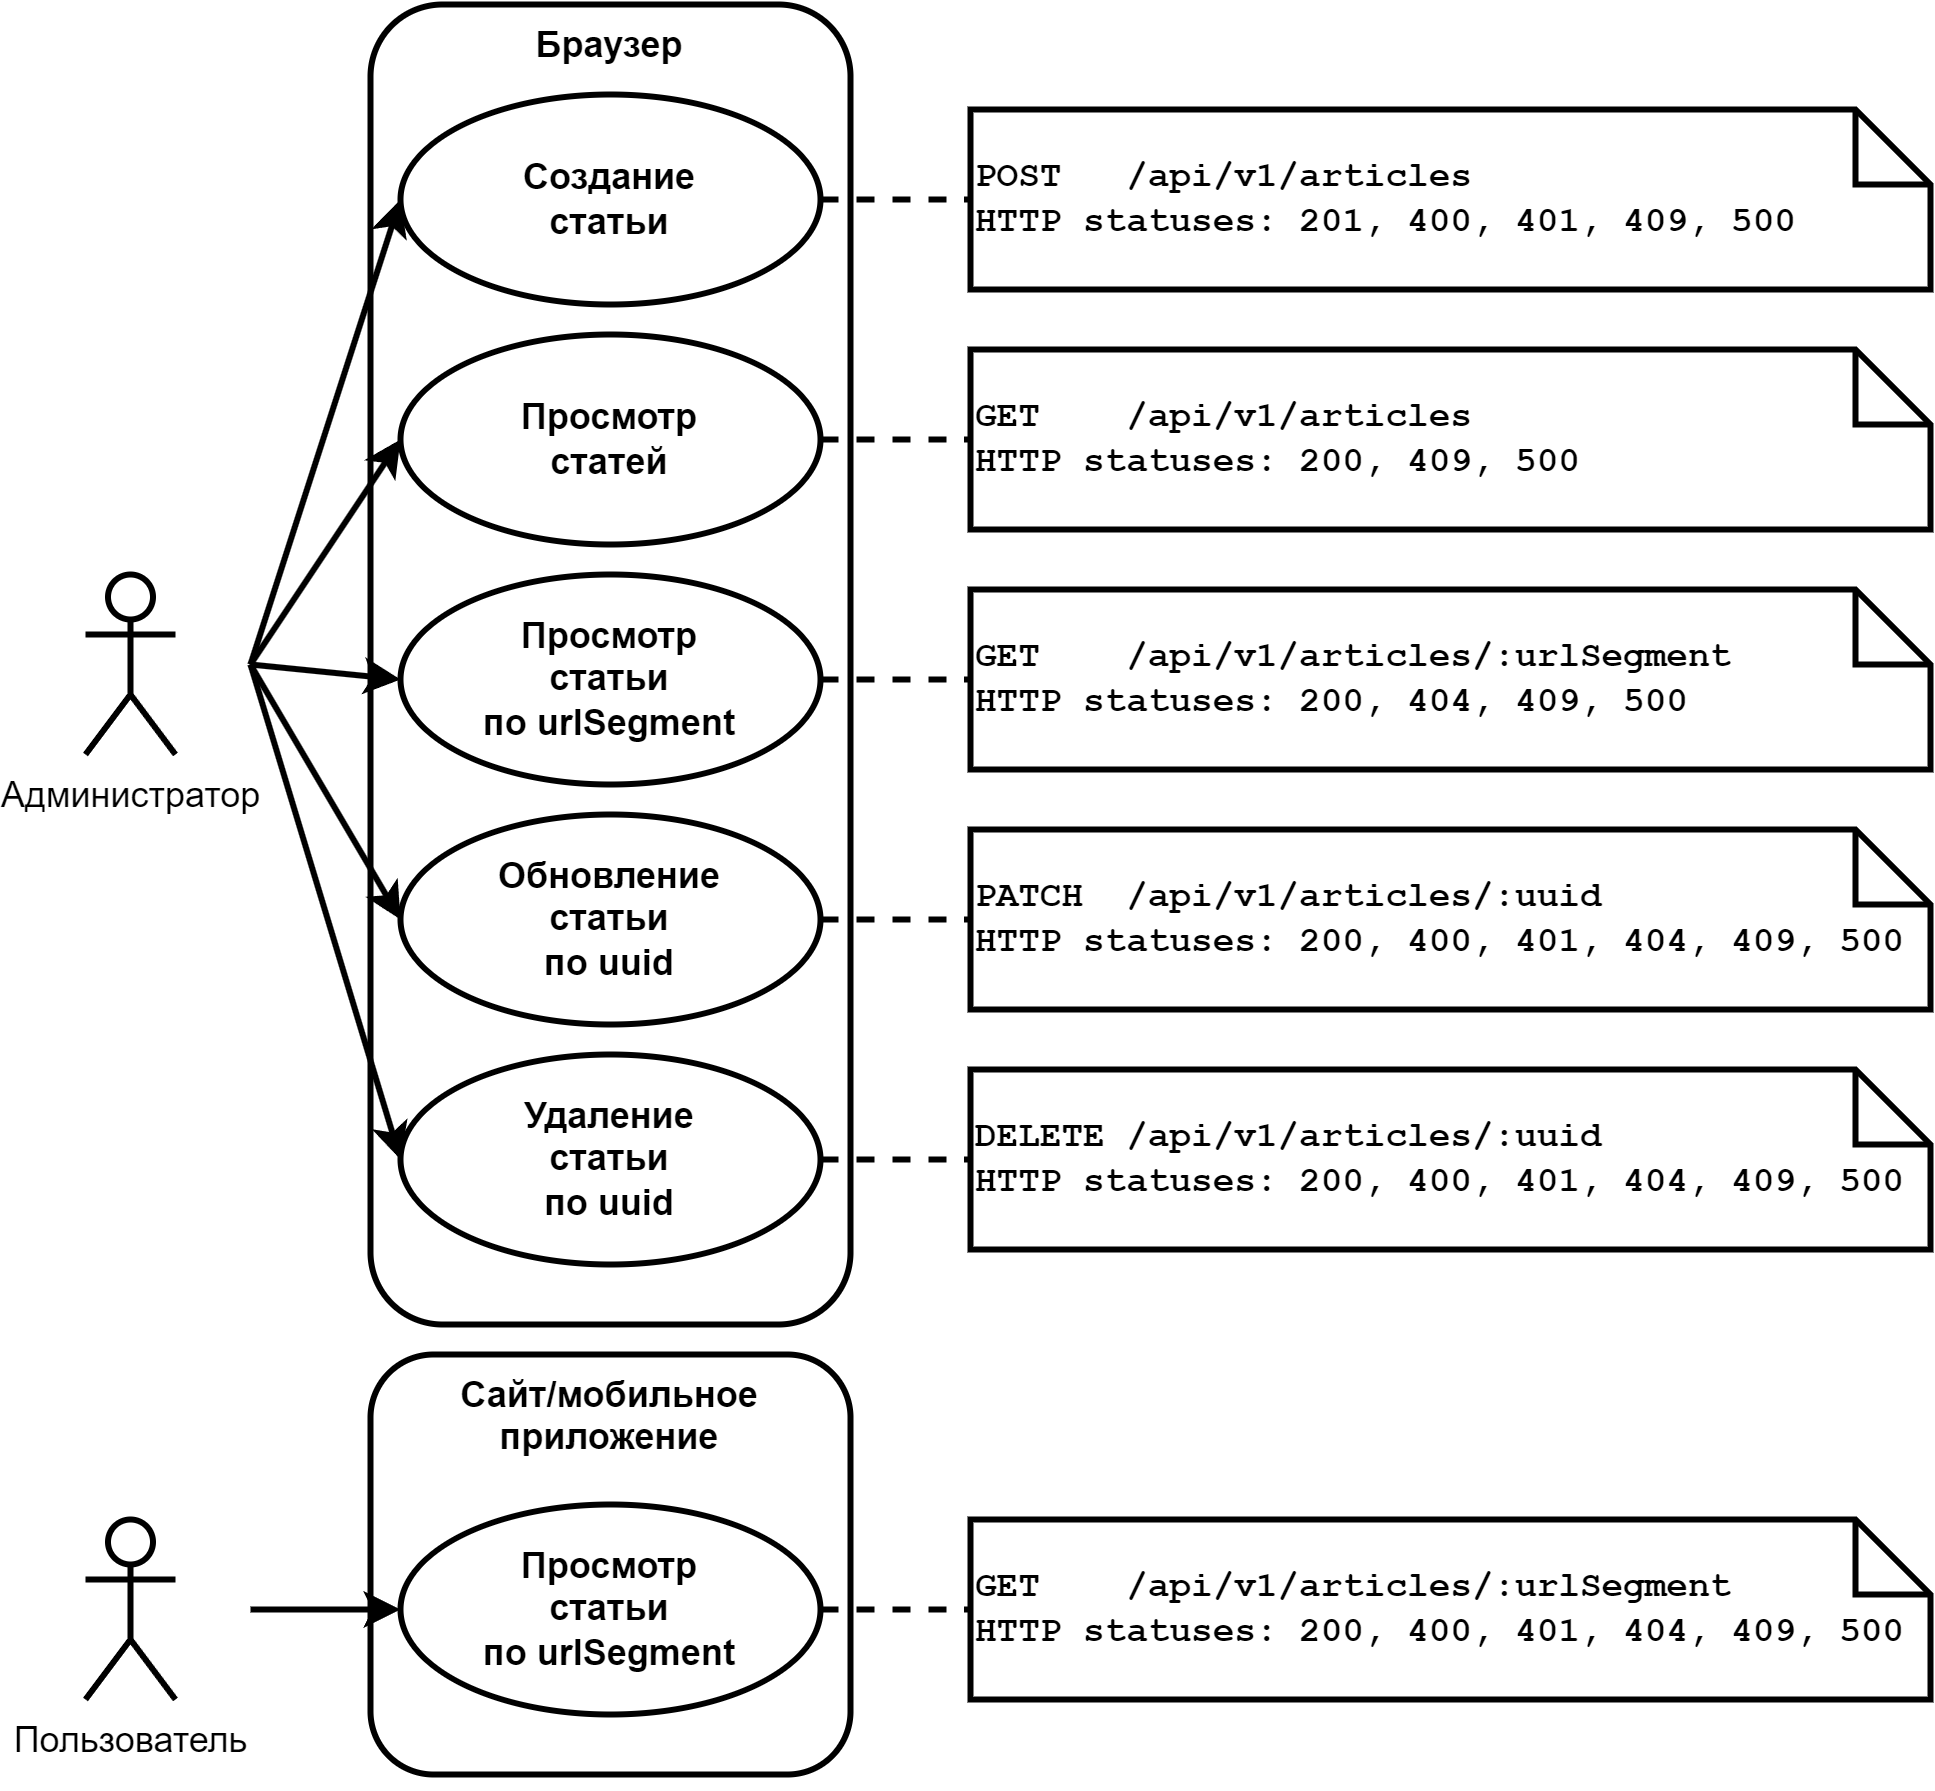
\includegraphics[height=7.5cm]
    {images/UML/UML_precedent_articles.png}

    \caption{Диаграмма прецедентов для манипуляции со статьями}

    \label{fig:UML_precedent_articles}
\end{figure}

% Таблица контактов (помощников) предназначена для хранения контактной информации организации,
% которая предоставляется пользователям для удобного взаимодействия.
% Здесь пользователи смогут найти все необходимые сведения и выбрать подходящий способ связи.
% Диаграмма прецедента <<Манипуляции с помощниками>> изображена на рисунке~\ref{fig:UML_precedent_helpres}.

% \begin{figure}[!htb]
%     \centering

%     \includegraphics[height=10cm]
%     {images/UML/UML_precedent_helpres.png}

%     \caption{Диаграмма прецедентов для манипуляции с помощниками}

%     \label{fig:UML_precedent_helpres}
% \end{figure}
